\documentclass{../sftex/sftex}

\usepackage{algorithm, algorithmic, gnuplottex, listings, parskip}

\newcommand{\binwds}[1]{\{0, 1\}^{#1}}
\renewcommand{\algorithmiccomment}[1]{\hfill $\triangleright$ #1}

\title{Power analysis of a hardware accelerated AES implementation}
\author{Gustavo Zambonin, Marcello Klingelfus}
\email{\{gustavo.zambonin,marcello.klingelfus\}@grad.ufsc.br}
\src{https://github.com/zambonin/epos-aes-docs}
\uniclass{Operating Systems II}
\classcode{UFSC-INE5424}

\begin{document}

\maketitle

\section{Motivation}

Devices in the Internet of Things are expected to interact with other machinery
in diverse situations. As such, threats to these communications should be
reduced or nullified altogether by means of protecting the hardware or software
from revealing critical information. However, these features may need expensive
calculations or precise timing. Hence, reduced energy consumption and increased
performance goals need careful consideration.

A \emph{cryptographic accelerator} can be used to help with these constraints,
operating in a more efficient way, through the calculation of steps of a
cryptographic algorithm on the hardware itself. Yet, using these features
requires a deep understanding of the processor used, and may not be available
or enabled on a given operating system.

We also point out that these implementations can be attacked non-invasively
through power analysis, \emph{i.e.} measuring power consumption and checking
for patterns in which secret data may be revealed. Ergo, \emph{constant-time}
algorithm implementations can be employed to prevent this undesired behaviour.
While these are usually very complex to implement, it is still useful to know
if current implementations using accelerators are prone to leak important data.

\section{Goals}

The underlying system-on-chip (SoC) powering EPOSMote III, called CC2538, is
derived from the ARM Cortex-M3 blueprint. It features hardware accelerators for
AES and RSA ciphers, and the SHA256 cryptographic hash
function~\cite{Texas:report:2013:may}. Poly1305, an AES-based message
authentication code, is used inside EPOS to achieve data authenticity and
integrity, as seen in~\cite{Resner:inproc:2015:feb}. Hence, it is desirable to
\emph{optimise the current implementation for the AES cipher}, making use of
the cryptographic cores available directly from the processor, as well as
\emph{profile its power usage} within a low-footprint, simplified EPOS
instance.

Optionally, it is beneficial to apply techniques to harden the code and making
it resilient to power analysis, as well as measure how deeply one may control
the hardware accelerated cryptographic directives, \emph{i.e.} if there are
only ``black-boxes'' available or separate steps for each cipher, since one can
more finely analyse the power consumption for these separate operations. An
example of this study can be seen in~\cite{Schwabe:inproc:2016:aug}.

\section{Methodology}

To reach our goal, we will first need to study and fully understand the AES
cipher in the context of CC2538, \emph{i.e.} how the cryptographic hardware
provided by EPOSMote III's SoC works. We will then implement a driver that uses
the hardware accelerated features for AES inside EPOS\@. Afterwards, its
correctness will be tested, and its performance measured against the previous
implementations. Finally, we will analyse its power consumption by means of
reducing the underlying operating system's noise with regards to background
tasks, modifying it accordingly (\emph{e.g.} replacing system components by
simpler alternatives, such as the thread scheduler).

\section{Tasks}

\begin{enumerate}
  \item Elaborate a detailed project plan;
  \begin{enumerate}
    \item Present a synopsis of the knowledge vital to understanding the
        project;
    \item Write on the project's progress periodically.
  \end{enumerate}
  \item Demonstrate the project's viability;
  \begin{enumerate}
    \item Use an external implementation that provides working examples for
        the AES cipher (suggestion:
          \href{https://github.com/contiki-os/contiki}{Contiki});
    \item Customize the traits file for a simple application, focusing on
        producing less background noise from EPOS\@;
    \item Manipulate the AES cryptographic core in the context of an EPOS'
        application;
    \item Describe the process and materials needed to execute a simple power
        analysis on the AES implementations.
  \end{enumerate}
  \item Implement a driver based on the cryptographic accelerator for AES on
      EPOS\@;
  \begin{enumerate}
    \item Provide a faster way to calculate AES operations in the form of a
        driver, with the current software implementation acting as fallback;
    \item Assert its correctness with
        \href{https://csrc.nist.gov/CSRC/media/Projects/Cryptographic-Algorithm-Validation-Program/documents/aes/AESAVS.pdf}{test
          vectors validated by NIST};
    \item Build tests in the context of the Poly1305 algorithm.
  \end{enumerate}
  \item Benchmark the previous AES implementation inside EPOS against code
      using hardware accelerated routines;
  \begin{enumerate}
    \item Create applications that measure the execution time for both
        implementations through repeated executions of the algorithm;
    \item Quantify the power consumption for both algorithms.
  \end{enumerate}
  \item Reduce the operating system footprint and measure the power profile
      for the hardware accelerated implementation;
  \begin{enumerate}
    \item Simplify the EPOS instance as much as possible for this particular
        setting through its traits file;
    \item Make use of an oscilloscope to profile the new implementation's
        inner workings;
    \item Optionally, analyse the software implementation as well.
  \end{enumerate}
  \item Compare all implementations and display practical results.
  \begin{enumerate}
    \item Simulate real, secure communications between motes, making use of
        the driver inside Poly1305.
  \end{enumerate}
\end{enumerate}

\section{Deliverables}

\begin{enumerate}
  \item Project plan (this document);
  \begin{enumerate}
    \item Update this page constantly with the project's advancements.
  \end{enumerate}
  \item Report consisting of a simple demonstration of technological viability;
  \begin{enumerate}
    \item Present, through the project plan, the concepts of cryptographic hash
        functions, message authentication codes, the AES cipher, and power
          analysis;
    \item Display any working mechanisms from the cryptographic accelerator
        inside EPOS through an application file;
  \end{enumerate}
  \item Code that talks to the AES cryptographic accelerator through EPOS\@;
  \begin{enumerate}
    \item Provide an API-compatible hardware accelerated implementation for the
        AES cipher with 128-bit keys;
    \item Feature Electronic Code Book (ECB) and Cipher Block Chaining (CBC)
        modes working through polling;
    \item Maintain the existing software implementation, as a fallback mode,
        for devices that do not provide the CC2538's cryptographic accelerator;
    \item Document the effort through the project plan;
    \item Optionally, implement interruption management for this driver;
    \item Optionally, add other AES modes, such as CBC-MAC (Cipher Block
        Chaining Message Authentication Code), CTR (Counter), GCM
          (Galois/Counter Mode) and CCM (Counter with CBC-MAC);
    \item Optionally, extend the key size to 192 and 256 bits.
  \end{enumerate}
  \item Report with performance comparison between software and hardware AES
    implementations on EPOS\@;
  \begin{enumerate}
    \item Compare the two implementations with stress testing, by means of
        repeated ciphering and deciphering, with the intent of measuring the
          execution time and power consumption;
    \item Graph these comparisons and exhibit these on the project plan.
  \end{enumerate}
  \item Report on power analysis, observed through an oscilloscope, for the new
    driver implementation;
  \begin{enumerate}
    \item Reduce EPOS' footprint by streamlining some of its core components,
        \emph{e.g.} the thread scheduler;
    \item Operate an oscilloscope with the aid of specially designed circuitry
        to observe the power consumption and check for information leaks;
    \item Register the experiment's results on the project plan.
  \end{enumerate}
  \item Project demonstration.
  \begin{enumerate}
    \item Show results obtained through a presentation to the class.
  \end{enumerate}
\end{enumerate}

\section{Schedule}

\begin{table}[htbp]
  \centering
  \begin{tabular}{lccccccccc}
    \textbf{Task}           & \textbf{30/04} & \textbf{07/05} & \textbf{14/05}
        & \textbf{21/05} & \textbf{28/05} & \textbf{04/06}
        & \textbf{11/06} & \textbf{18/06} & \textbf{25/06} \\
    Task 1 --- Project plan   & E1             &                &
        &                &                &
        &                &                &                \\
    Task 2 --- Viability      & E1             &                &
        &                &                &
        &                &                &                \\
    Task 3 --- AES driver     & x              & x              & E2
        &                &                &
        &                &                &                \\
    Task 4 --- Benchmarks     &                &                & x
        & x              & E3             &
        &                &                &                \\
    Task 5 --- Power analysis &                &                & x
        & x              & x              & x
        & E4             &                &                \\
    Task 6 --- Demonstration  &                &                &
        &                &                &
        & x              & x              & E5             \\
  \end{tabular}
\end{table}

\section{Basic concepts}

We start by explaining the concepts related to cryptography needed to
understand the body of this work. Namely, we talk about cryptographic hash
functions, message authentication codes (MACs), the AES cipher, an example of
MAC called Poly1305, and power analysis. Afterwards, we show preliminary
results on the EPOSMote III platform and EPOS that allow us to demonstrate the
technological viability of this project.

\subsection{AES --- Advanced Encryption Standard}

AES is a block cipher that operates with key sizes of 128, 192 and 256 bits on
a state matrix of $4 \times 4$ words. The words are polynomials of a Galois
field with order 256, chosen for its easy computational representation and
solid mathematical basis. It is an iterative cipher, featuring repeated
applications (rounds) of four basic operations on the state matrix.

Consider the following pseudocode for the encryption algorithm. Denote $n$ as
the size of key, $\ell = \frac{n}{32}$, $n_r$ as the number of rounds ($n_r =
10$ if $n = 128$, $n_r = 12$ if $n = 192$, $n_r = 14$ if $n = 256$) and $A$ as
the state matrix.

\begin{algorithm}
  \begin{algorithmic}
    \REQUIRE{}  $m \in \binwds{128}, \enspace
      K \in \cup_{n \in \{128, 192, 256\}} \binwds{n}$
      \COMMENT{plaintext and key}
        \ENSURE{}  $c \in \binwds{128}$ \COMMENT{ciphertext}

    \STATE{}  $A \leftarrow m$
    \STATE{}  $\{k_{0} \dots k_{(n_{r} + 1) \cdot \ell}\}
      \leftarrow \textsc{KeyExpansion}(K)$
    \STATE{}  $A \leftarrow \textsc{AddRoundKey}(A,
      \{k_{0}, \dots, k_{\ell - 1}\})$

    \FOR{$i \leftarrow 1$ até $n_{r} - 1$}
      \STATE{}  $A \leftarrow \textsc{SubBytes}(A)$
      \STATE{}  $A \leftarrow \textsc{ShiftRows}(A)$
      \STATE{}  $A \leftarrow \textsc{MixColumns}(A)$
      \STATE{}  $A \leftarrow \textsc{AddRoundKey}(A,
        \{k_{i \cdot \ell}, \dots, k_{(i + 1) \cdot \ell - 1}\})$
    \ENDFOR{}

    \STATE{}  $A \leftarrow \textsc{SubBytes}(A)$
    \STATE{}  $A \leftarrow \textsc{ShiftRows}(A)$
    \STATE{}  $A \leftarrow \textsc{AddRoundKey}(A,
      \{k_{n_{r} \cdot \ell}, \dots, k_{(n_{r} + 1) \cdot \ell - 1}\})$

    \STATE{}  $c \leftarrow A$
  \end{algorithmic}
  \caption{AES ciphering process.}
\end{algorithm}

We briefly discuss the routines mentioned above and refer
to~\cite{Daemen:book:2002} for detailed explanations.

\begin{itemize}
  \item \textsc{SubBytes}: substitute every element of $A$ for its
      corresponding value inside a substitution-box (S-box, built from the
        multiplicative inverse of elements in the Galois field along with an
        affine transformation), with the intent of concealing the relationship
        between key and ciphertext;
  \item \textsc{ShiftRows}: shift every row of $A$ by a fixed amount, with the
      intent of scattering the values of the state matrix, avoiding the
        independent encryption of columns;
  \item \textsc{MixColumns}: multiply every column of $A$ by a specific
      polynomial and apply modular reduction, achieving further diffusion;
  \item \textsc{AddRoundKey}: combine $A$ with the round key through an
      exclusive or operation;
  \item \textsc{KeyExpansion}: derives a set of words from the key so these can
      be used in every round, through the use of efficient and non-linear byte
        operation, preventing localization of patterns that can reveal the
        master key.
\end{itemize}

AES is an example of symmetric cryptography, \emph{i.e.} it uses a single key
for encryption and decryption. Hence, the routines above need to be easily
inverted, but only if one provides the master key. We present the pseudocode
for the decryption algorithm and discuss the new routines.

\begin{algorithm}
  \begin{algorithmic}
    \REQUIRE{}  $c \in \binwds{128}, \enspace
      K \in \cup_{n \in \{128, 192, 256\}} \binwds{n}$
      \COMMENT{ciphertext and key}
    \ENSURE{}  $m \in \binwds{128}$ \COMMENT{plaintext}

    \STATE{}  $A \leftarrow c$
    \STATE{}  $\{k_{0} \dots k_{(n_{r} + 1) \cdot \ell}\}
      \leftarrow \textsc{KeyExpansion}(K)$
    \STATE{}  $A \leftarrow \textsc{AddRoundKey}(A,
      \{k_{n_{r} \cdot \ell}, \dots, k_{(n_{r} + 1) \cdot \ell - 1}\})$

    \FOR{$i \leftarrow n_{r} - 1$ até $1$}
      \STATE{}  $A \leftarrow \textsc{InvShiftRows}(A)$
      \STATE{}  $A \leftarrow \textsc{InvSubBytes}(A)$
      \STATE{}  $A \leftarrow \textsc{AddRoundKey}(A,
        \{k_{i \cdot \ell}, \dots, k_{(i + 1) \cdot \ell - 1}\})$
      \STATE{}  $A \leftarrow \textsc{InvMixColumns}(A)$
    \ENDFOR{}

    \STATE{}  $A \leftarrow \textsc{InvShiftRows}(A)$
    \STATE{}  $A \leftarrow \textsc{InvSubBytes}(A)$
    \STATE{}  $A \leftarrow \textsc{AddRoundKey}(A,
      \{k_{0}, \dots, k_{\ell - 1}\})$

    \STATE{}  $m \leftarrow A$
  \end{algorithmic}
  \caption{AES deciphering process.}\label{alg:aesdecrypt}
\end{algorithm}

\begin{itemize}
  \item \textsc{InvShiftRows}: shift every row of $A$ by a fixed amount,
      inverting the correspondent diffusion on the encryption algorithm;
  \item \textsc{InvSubBytes}: substitute every element of $A$ by its
      corresponding element on the inverse S-box (obtained by applying the
        inverse of the affine transformation and then taking the multiplicative
        inverse in the Galois field);
  \item \textsc{InvMixColumns}: multiply every columns of $A$ by a specific
      polynomial (the multiplicative inverse of the polynomial for the
        corresponding step).
\end{itemize}

\subsection{Cryptographic hash function}

Consider two sets, $X$ and $Y$, with words of length $m$ and $n$ respectively,
such that $m > n$. A function $H : X \longrightarrow Y$ can be defined as a
hash (or compressing) function, since elements of $Y$ are generally called
hashes or digests. $H$ is defined to be deterministic and computationally
efficient. To consider $H$ as cryptographic, other restrictions are taken into
account:

\begin{itemize}
  \item Preimage resistance, \emph{i.e.} the function cannot be inverted
      efficiently;
  \item Second preimage resistance, \emph{i.e.} given $m_0 \in X$, it should
      not be computationally feasible to find a different $m_1 \in X$ such that
        their hashes are equal;
  \item Collision resistance, \emph{i.e.} it should not be computationally
      feasible to find any two distinct messages in X with equal hashes;
  \item Presence of the avalanche effect, wherein a single bit change on the
      input should change approximately half of the bits on the output.
\end{itemize}

Note that collision resistance implies second preimage resistance. In the
former, an attacker may choose any two messages from $X$, whereas in the latter
one message is fixed and cannot be changed. Hence, it is said that second
preimage resistance is much stronger as a security requirement.

\subsection{Message authentication code}

To create a message that has not only integrity, but also authenticity
(\emph{i.e.} one can verify if it really came from a specified sender), a MAC
construction has to be employed. It authenticates a message by signing it with
a symmetric key. Consequently, there must be a way for two (or more) entities
to agree on a key. It follows that, if a key is shared between multiple devices
(\emph{e.g.} a sensor network), every device that can verify a MAC can also
generate other MACs. It consists of three algorithms that can be computed
efficiently:

\begin{itemize}
  \item Key generation, where on input of a security parameter $n$ (usually a
      large enough integer), a random key is produced from a key space
        (\emph{e.g.} the set of all binary words of length $n$);
  \item Signature generation, where on input of a key and any message, it
      produces a tag (a short name for an authenticated message);
  \item Signature verification, where on input of a tag and a key, it returns a
      Boolean value on whether the tag was created with that key.
\end{itemize}

Note that this construction should be able to resist forgeries, that is, it
should be computationally unfeasible to guess the MAC for messages that were
created with an unknown key. We give an example of MAC algorithm in the form of
Poly1305-AES and refer to the original paper for detailed
explanations~\cite{Bernstein:inproc:2005:feb}. It is sufficient to know that
Poly1305 is a polynomial evaluation modulo $2^{130} - 5$, with the following
parameters: a secret key with two values (the key for AES and a random integer
with special properties), an unique number (nonce) to be encrypted using AES,
and the message to be tagged. The underlying security of the algorithm is based
on the nonce encryption mechanism. Observe that AES may be replaced at any time
by another cipher.

\subsection{Power analysis}

A cryptographic algorithm is not only required to present a solid mathematical
proof, but also implementations that can resist side-channel attacks. Secret
information may be retrieved if it can be finely measured and physically
exploited. Cache and timing attacks, introduction of faults by placing the
device under extreme conditions, acoustic and electromagnetic monitoring etc.
are various forms of side-channel attacks. We focus on the concept of power
analysis, introduced in~\cite{Kocher:inproc:1999:aug}, in which the power
consumption may be studied to obtain sensitive data from a given device, and
further restrict our scope to simple power analysis, where one can directly
measure and visualize the power consumption collected from cryptographic
operations.

Consider the example of a RSA cipher, that works with multiplications and
squaring modulo prime numbers. These can be distinguished by looking at the
measurements through a standard digital oscilloscope. Statistical analysis of
the values and removal of background electrical noise may be required to
enhance the observation results.

\section{Technological viability}

We now introduce these concepts to the EPOS environment. First, to ensure that
a meaningful test bench is used to test the new driver implementation, we
created an application out of the \verb!src/component/poly1305_test.cc! file
and executed it to ensure the software implementations for the algorithms work
correctly, getting positive results and a meaningful execution time. A simple
task to prove the viability for the driver implementation is to actually
manipulate the cryptographic core. Hence, many definitions in the form of
memory addresses for registers and function prototypes had to be migrated to
EPOS, from the \href{http://www.ti.com/tool/CC2538-SW}{official driver library}
provided by Texas Instruments. We created a dependency graph of the files from
that library, starting by
\verb!cc2538_foundation_firmware_1_0_1_0/driverlib/.../aes_example.c!. We found
out that hardly any files are needed, namely (folder names omitted for
clarity):

\begin{itemize}
  \item source files are \verb!aes.c! (AES driver), \verb!cpu.c! (instruction
      wrappers), \verb!interrupt.c! (driver for the NVIC --- Nested Vectored
        Interrupt Controller) and \verb!sys_ctrl.c! (driver for the system
        controller);
  \item header files are, in addition to corresponding files for each source
      above, \verb!hw_aes.h!, \verb!hw_flash_ctrl.h!, \verb!hw_nvic.h!,
        \verb!hw_sys_ctrl.h! (addresses and constants for registers that manage
        the AES driver, flash ROM, NVIC and system controller, respectively),
        \verb!hw_ints.h! (defines for types of interruptions) and
        \verb!hw_types.h! (common types and macros for hardware access).
\end{itemize}

Hence, we moved these files to the EPOS codebase and adapted them
accordingly to compile a test application. We present an application that
manages to enable the AES core, and discuss the code in detail.

\begin{lstlisting}[language=C++,numbers=none]
  #include <utility/aes-hw/aes.h>
  #include <utility/aes-hw/hw/hw_sys_ctrl.h>
  #include <utility/ostream.h>

  using namespace EPOS;
  OStream cout;

  typedef struct {
    unsigned char ui8AESKey[16];            // stores the Aes Key
    unsigned char ui8AESKeyLocation;        // location in Key RAM
    unsigned char ui8AESBuf[16];            // input buffer
    unsigned char ui8AESExpectedOutput[16]; // expected results
    unsigned char ui8IntEnable;             // set to true to enable interrupts
  } tAESExample;

  tAESExample sAESexample[] = {
      {{0x00, 0x00, 0x00, 0x00, 0x00, 0x00, 0x00, 0x00, 0x00, 0x00, 0x00, 0x00,
        0x00, 0x00, 0x00, 0x00},
       0,
       {0x6c, 0x5f, 0x51, 0x74, 0x53, 0x53, 0x77, 0x5a, 0x5a, 0x5f, 0x57, 0x58,
        0x55, 0x53, 0x06, 0x0f},
       {0x83, 0x78, 0x10, 0x60, 0x0e, 0x13, 0x93, 0x9b, 0x27, 0xe0, 0xd7, 0xe4,
        0x58, 0xf0, 0xa9, 0xd1},
       false},
  };

  int main() {
    // enable AES peripheral
    HWREG(SYS_CTRL_RCGCSEC) = 0x00000002;

    // mimic start of aes.cc@AESLoadKey
    unsigned char *pui8Key = sAESexample[0].ui8AESKey;
    static unsigned int ui32temp[4];
    unsigned char *pui8temp = (unsigned char *)ui32temp;
    unsigned char i;

    // key address needs to be 4 byte aligned
    for (i = 0; i < KEY_BLENGTH; i++) {
      pui8temp[i] = pui8Key[i];
    }

    // configure master control module
    // enable DMA path to the key store module
    HWREG(AES_CTRL_ALG_SEL) = 0x00000001;

    // clear any outstanding events
    HWREG(AES_CTRL_INT_CLR) = 0x00000001;

    // configure key store module (area, size)
    // 128-bit key size
    HWREG(AES_KEY_STORE_SIZE) = 0x00000001;

    // enable keys to write (e.g. Key 0)
    HWREG(AES_KEY_STORE_WRITE_AREA) = 0x00000001;

    // configure DMAC
    // enable DMA channel 0
    HWREG(AES_DMAC_CH0_CTRL) = 0x000000001;

    // base address of the key in ext. memory
    cout << hex << "AES_DMAC_CH0_EXTADDR before writing: "
      << HWREG(AES_DMAC_CH0_EXTADDR) << endl;
    HWREG(AES_DMAC_CH0_EXTADDR) = (unsigned int)pui8temp;
    cout << hex << "AES_DMAC_CH0_EXTADDR after writing: "
      << HWREG(AES_DMAC_CH0_EXTADDR) << endl;

    // total key length in bytes (e.g. 16 for 1 x 128-bit key)
    HWREG(AES_DMAC_CH0_DMALENGTH) = 0x10;

    return 0;
  }
\end{lstlisting}

This implementation follows the directives in~\cite[Sec.
22.2.5.4.2.1]{Texas:report:2013:may} and can actually write the base key
address to the \verb!AES_DMAC_CH0_EXTADDR! register, with value
\verb!0x20000050!. The module is enabled by setting the second bit of the
\verb!SYS_CTRL_RCGCSEC! register, as per~\cite[Sec. 7.7.12, pp.
207]{Texas:report:2013:may}. Afterwards, DMA is enabled, and the module can
already fetch the key from external memory, finally writing it to the key store
(a protected memory region). If the module is disabled, the base key address
will not be written at all. Note that \verb!aes_example.c! features both
interrupt and polling implementations; the interrupt drivers may not be needed
if polling is used exclusively, thus reducing the amount of code needed to
port. Additionally, it showcases only ECB (Electronic Code Book) mode, whereas
other modes can be used, according to~\cite[Sec.
22.2.1.1.3]{Texas:report:2013:may}.

Finally, we briefly discuss how to measure the power consumption through an
oscilloscope. Preliminary discussion showed that an \emph{amplifier circuit} is
needed. One needs to mangle a USB-microUSB cable, acting as power for the
EPOSMote III, to insert a shunt resistor and actually read tension from the
current passing through the cable. Then, since the signal is too weak to be
captured by the scope, one will need an
\href{http://www.ti.com/product/TL074}{operational amplifier}, some resistors
(according to \href{http://epos.lisha.ufsc.br/dl675?display}{this description})
and a protoboard to implement an amplifier circuit. Finally, when the scope is
able to sense it, the measurements can be taken (this circuit design is subject
to changes). One can also disable certain parts of the SoC by making use of the
deep sleep feature~\cite[Sec. 3.5.1, pp. 132]{Texas:report:2013:may}, and
simplify the application's traits file, to reduce background noise.

\section{Driver implementation}

One of the core features of EPOS is that it supports multiple computer
architectures. Hence, one needs to ensure that applications that need to
instantiate the AES cipher may do so at any time even if there is no
cryptographic accelerator available. Therefore, the current software
implementation is kept for compatibility and comparison purposes, and the
challenge lies in adding a hardware driver in such a way that no conflicts are
caused, and the operating system uses hardware availability as criteria to
choose the correct implementation.

In the last section, examples were presented that already included directives
to talk directly with the cryptographic core, but their backbone was not
correctly integrated with the operating system and lacked generality and scope
(since the AES cipher is used on a core component of EPOS, the Trustful
Space-Time Protocol). Additionally, the file dependency graph created did not
consider that there could be low-level features already integrated on EPOS,
such as dealing with the \verb!SYS_CTRL! registers.

With these issues in mind, files and functions from the former example were
deemed irrelevant. As per \verb!aes_example.c!, setting the clocks to 32MHz is
not needed since EPOS already runs in that frequency, according to the source
code located in \verb!src/machine/cortex/emote3_init.cc!. Enabling the
peripheral may be achieved through a write to the \verb!SYS_CTRL_RCGCSEC!
register (or variants if the device is on sleep, or deep sleep mode), and
inside EPOS, this is done through \verb!power_aes(const Power_Mode&)!, called
from \verb!src/machine/cortex/machine_init.cc!.

All declarations and definitions for the driver are inside the
\verb!include/machine/cortes/aes.h! mediator file. This implementation is only
compiled (and consequently, the peripheral enabled) if EPOS is compiled with a
Cortex-M3 target, through the use of static metaprogramming in the mediator
file. The software implementation from \verb!include/utility/aes.h! is used
instead. Implementation hints were taken from the firmware provided by Texas
Instruments and heavy use of the manual in~\cite{Texas:report:2013:may} was
made to ascertain semantics of the code. Electronic Code Book and Cipher Block
Chaining modes are supported, with the key size of 128 bits, as needed by
EPOS\@. Other modes and key sizes may be added with non-trivial modifications
to the code.

API compatibility is provided through the use of default parameters, but
altogether, six parameters can be passed to \verb!encrypt! and \verb!decrypt!
methods: pointers to the key, input data, output data, initialization vector,
mode of operation (as per a simple enumeration that maps to the
\verb!AES_AES_CTRL! register options) and key store location (eight 128-bit
available memory areas). As in the software implementation, AES-ECB-128 mode of
operation is the default. Tests with the standalone cipher and a Poly1305-AES
instantiation are provided in the form of the files \verb!app/aes_test.cc! and
\verb!app/poly1305_test.cc!, respectively. These are originally located inside
the \verb!src/component! folder, but failed to compile, and are now fixed. We
refer to the branch containing the modified codebase for implementation
details: \href{https://epos.lisha.ufsc.br/svn/makers/aes-driver/}{aes-driver}
or its \href{https://github.com/zambonin/epos-aes-driver}{mirror} on GitHub.

Furthermore, messages with arbitrary length are now supported, featuring a
common padding strategy described in~\cite{Kaliski:report:1998:mar} if the
length is not a multiple of the block size. It is reasonable to consider
implementing this feature, since the execution time for ciphering and
deciphering various amounts of blocks can be finely measured, enabling a deeper
understanding of the cost associated with the cryptographic core setup and the
operation modes themselves. We point out that~\cite[Sec.
22.2.4]{Texas:report:2013:may} presents the basis for performance calculations.
In special, we emphasize the footnotes 1 and 2 from~\cite[Table
22--88]{Texas:report:2013:may}:

\begin{itemize}

  \item ``The performance assumes full programming of the engine, loading keys
      and setting up the DMA engine via the DMA slave. If the context is reused
        (mode and/or keys) the performance is increased. The maximum number of
        cycles overhead per packet is between 100 and 150 for the various modes
        and algorithms.''

   \item (\ldots) ``The performance scales linearly with the clock frequency.''

\end{itemize}

\section{Benchmarks}

To achieve meaningful performance results, some metrics such as execution time
and energy consumption were considered. However, time measurements were not
significant, and to achieve relevant energy metrics, the apparatus discussed in
the section about power analysis would have to be built. Hence, these
quantities will be discussed on any account, and need not be measured now.
Performance-oriented algorithm implementations are generally measured in
instruction cycles, arguably the strictest operational criteria, and these may
be consequently translated to the aforementioned metrics. Ergo, we choose
instruction cycles for our measurements.

Accordingly, we make use of the Cortex-M3 integrated system timer, SysTick,
which provides a 24-bit counter, useful for various tasks. We program this
timer in accordance to~\cite[Sec. 3.4]{Texas:report:2013:may}, namely by
enabling it through the \verb!STCTRL! register, loading the \verb!STRELOAD!
register with the maximum counter possible (that is, $2^{24} - 1$), and reading
the \verb!STCURRENT! register whenever desired to check how many cycles were
counted. We note that this strategy is already implemented inside
\verb!include/machine/cortex/timer.h!.

We enclosed \verb!crypt(...):include/machine/cortex/aes.h! with these
directives and took notes of a dozen executions for various message sizes,
ciphered and deciphered with ECB and CBC\@. More executions were not needed,
since the clock counts varied by approximately 50 cycles.

\begin{figure}[ht]
  \centering
  \begin{gnuplot}[terminal=pdf]
    set key autotitle columnhead
    set key bottom inside
    set title "Execution data from AES driver for CC2538"
    set xlabel "Message size (bytes)"
    set logscale x
    set grid
    set ylabel "Instruction cycles"
    plot for [col=2:5] "support/cycles-aes.txt" \
      using 1:col:xtic(1) with linespoints
  \end{gnuplot}
\end{figure}

Note that this graph presents a logarithmic scale, but the message size
increases exponentially. Hence, it is useful to look at the delta measurements
between each pair of variables to check if this visual representation is
inappropriate. Indeed, we note that the differences double with each step,
ergo, this behavior can be considered linear. However, it is useful to look at
the variations with small message sizes, emphasized in this scale. We firmly
believe that this behavior can be explained by the setup cost for the
cryptographic core, again based on the delta measurements, and confirm the
first footnote from~\cite[Table 22-88]{Texas:report:2013:may}. Finally, we
link to a \href{https://epos.lisha.ufsc.br/dl875?display}{similar graph} with
measurements in microseconds.

In~\cite[Table 1]{Schwabe:inproc:2016:aug}, the total cost for an AES-128
simple encryption and decryption routine is $\sim 2750$ cycles. Our
implementation is almost twice as fast, depending on the chosen operation mode,
simply due to the cryptographic core usage. The cost for the naïve AES software
implementation inside EPOS is not shown on the graph for simplicity. However,
the measurements showed $\sim 14000$ and $\sim 20000$ cycles for encryption and
decryption using ECB mode, respectively. Therefore, it can be argued that our
hardware implementation may be used to save energy and increase performance.

\section{Power analysis}

According to the discussion on previous settings, an amplifier circuit was
built to correctly measure the power consumption of an EPOSMote III board, with
the intent of observing any patterns that may rise when ciphering data through
the aforementioned AES implementations. The circuit description cited above was
found to be overly complex, and hence, it was thoroughly simplified. We explain
the rationale to construct this circuit as follows. Since these measurements
need not be extremely precise, one can introduce new circuitry to the monitored
system without concerns. However, note that these can add noise or dissipate
power, which may not be desirable.

The first part of the circuit, a current sensor, is achieved by placing a shunt
resistor in series with the monitored system. The electric tension, or voltage,
generated by this apparatus can then be measured by an operational amplifier.
With help and materials supplied by LISHA, we amplify (and invert) the EPOSMote
III input current in 62x. \verb!RSHUNT!, \verb!R1! and \verb!R2! are,
respectively, 100$\Omega$, 1k$\Omega$ and 62k$\Omega$ resistors. The \verb!U1!
unit is a \href{http://www.ti.com/product/UA741}{UA741} operational amplifier,
powered by a symmetric $\pm$12V power supply connected to the \verb!VCC-! and
\verb!VCC+! pins. A picture of the new circuit may be checked
\href{https://epos.lisha.ufsc.br/dl821?display}{here}. Tektronix TDS-2024B
oscilloscope probes were installed on the output of this circuit, and first
measurements showed a high amount of electrical noise on the current. Hence, a
100 nF / 100 VDC capacitor was added in parallel to the shunt resistor and
other circuitry. Finally, we successfully measured the power consumption of
both software and hardware AES implementations. A picture of the oscilloscope
being used can be checked
\href{https://epos.lisha.ufsc.br/dl824?display}{here}.

Ciphering and deciphering of $2^{10}$ randomized messages of 16 bytes for both
ECB and CBC modes were interpreted by the oscilloscope. A back of the envelope
calculation suggests around $\sim 2.2$ seconds for this process to complete
entirely in the case of the software implementation. The new driver would take
a fifth of a second to execute an equivalent test bench, as well as optimizing
the existing test bench through the use of techniques such as loop unrolling to
reduce the overhead for execution of additional logic. This is shown through
the data sets reported by the oscilloscope and pictured below, in which the
``valleys'' are consistent with the execution of the image programmed into the
board. Note the aforementioned reduction in execution time. The randomized
messages strategy prevents a fair energy consumption comparison, but highlights
an irregular usage of energy, suggesting that both implementations may be weak
against side-channel attacks.

\begin{figure}[ht]
  \centering
  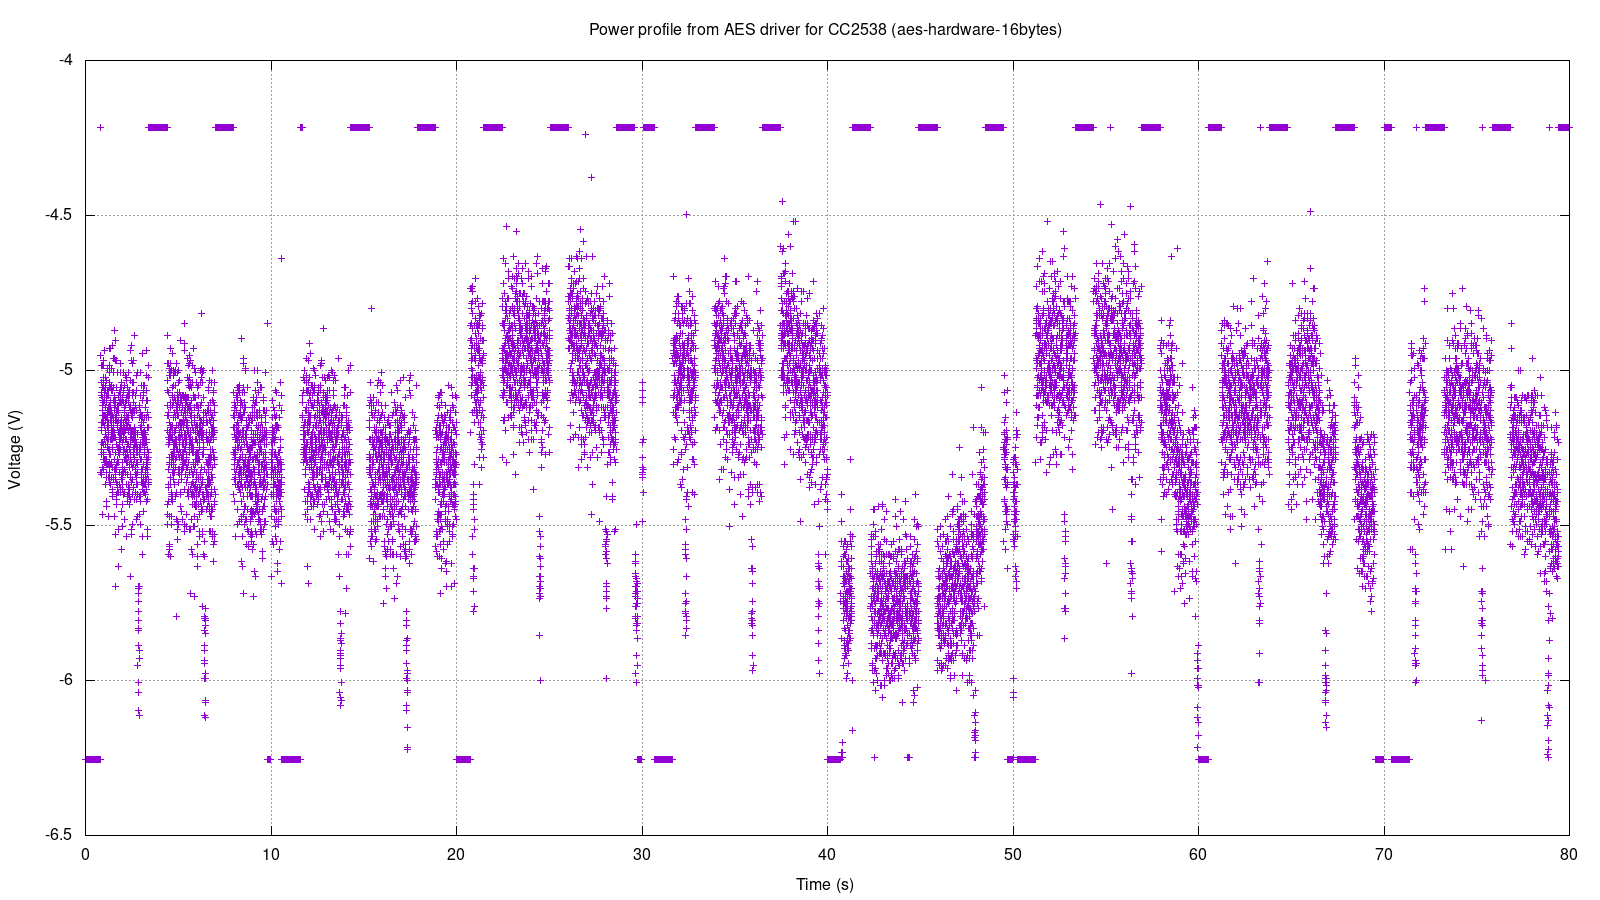
\includegraphics[width=\textwidth]{support/aes-hardware-16bytes.png}
  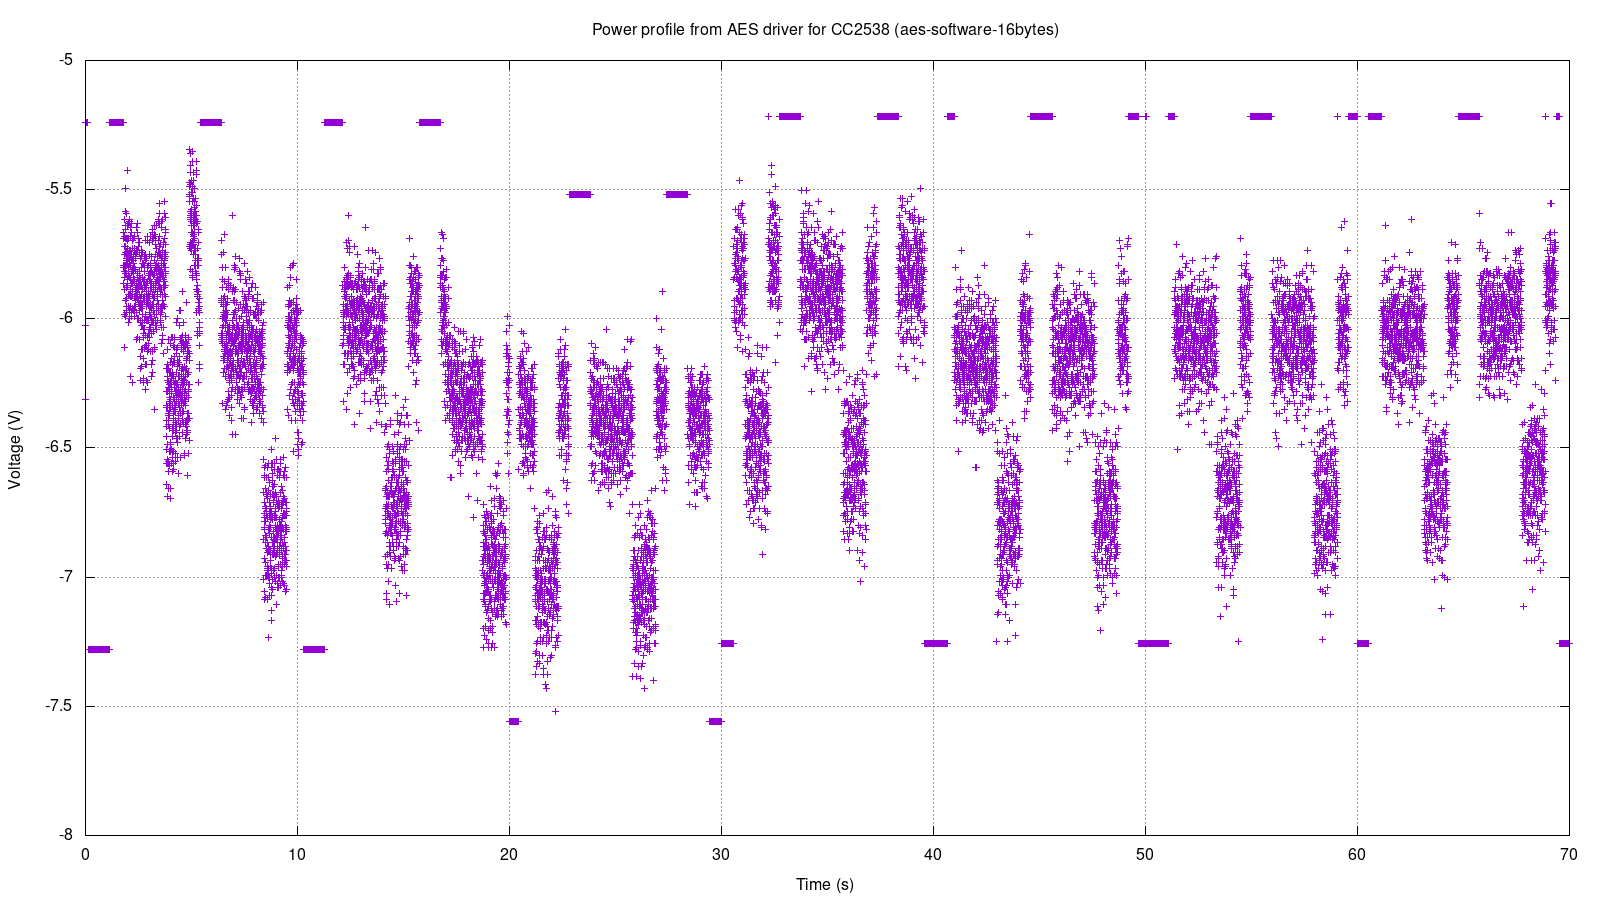
\includegraphics[width=\textwidth]{support/aes-software-16bytes.png}
\end{figure}

Further measurements were made with message lengths of 128 and 1024 bytes,
unsupported by the software cipher. However, these show an expected increase in
execution time and energy consumption, the latter incorrectly measured by the
device used due to lack of precision. For reproducibility and consulting
purposes, data and images produced directly by the oscilloscope are located on
the SVN branch. Repeated ciphering of the same test vector may be used as a
strategy to compare energy consumption for both implementations. Additionally,
it would be useful to ignore events such as board power up and power down. This
can be achieved through the oscilloscope's external trigger input connected to
a GPIO pin on the EPOSMote III board, activated and deactivated as soon as the
test bench starts and ends, respectively.

\section{Results and future works}

We discuss the results and limitations for this work, and present suggestions
for future projects with regards to side channel attacks and hardware
implementations of cryptographic algorithms in the context of EPOS and EPOSMote
III\@. First, we provide a fully functional, API-compatible, hardware
accelerated AES implementation for the CC2538 SoC, that amounts to a
twenty-fold increase in performance and decrease in energy consumption,
according to the number of instruction cycles. Consequently, the possibility of
timing attacks is greatly reduced, for the difficulty in getting relevant data
for key extraction is increased.

Available AES implementations are chosen according to target hardware through
the use of static metaprogramming and hardware mediators. Furthermore,
deprecated test benches in the EPOS codebase were rewritten and added as
test applications. In special, we note that all components that were already
using the AES cipher, such as TSTP, are untouched. Additionally, the high
maintainability of the driver codebase allows for the easy integration of
new AES modes, interruption management and extension of key sizes, listed as
optional goals above.

We also note that the provided AES software implementation may be susceptible
to cache attacks, since naïve utilization of a static array providing the S-box
constants is featured in the implementation. Moreover, it does not contain any
countermeasures to achieve constant-time operations when ciphering or
deciphering. It would also be the main target of an attacker, since its reduced
performance leads to more data being leaked.

Finally, we propose a rationale to proceed with a more intricate power analysis
of the available AES cipher implementations. Making use of dedicated hardware
for side channel attacks, such as
\href{https://github.com/newaetech/chipwhisperer}{ChipWhisperer}, or highly
sensitive equipment, \emph{e.g.} expensive oscilloscope and probes or
\href{https://web.archive.org/web/20170621162219/satoh.cs.uec.ac.jp/SASEBO/en}{
specialized boards}, is indeed required to achieve retrieval of meaningful
power traces. Furthermore, complex techniques such as correlation power
analysis, itself a form of differential power analysis, are generally employed
in the literature~\cite{Biryukov:inproc:2017:jul} and will prove useful in this
endeavor.

\bibliographystyle{alpha}
\bibliography{wiki}

\end{document}
